\documentclass[22pt]{beamer}
\usepackage[orientation=portrait, size=custom, width=91.44, height=60,scale=1.2]{beamerposter} % 36in*2.5 = 90cm
\usepackage[absolute,overlay]{textpos}
\usepackage{bookmark} %pdflatex says to use this to avoid errors...
\usepackage{graphicx} %for including images
\graphicspath{{figs/}} %location of images
\usepackage{wrapfig} %wrap text around the images
\usepackage{listingsutf8}    %package for code environment; use this instead of verbatim to get automatic line break; use this instead of listings to get (•)
\usepackage{amsmath}
\usepackage{gensymb}
\usepackage[export]{adjustbox}
\usepackage[skins,theorems]{tcolorbox}
\usepackage{pgfplots}
\usepackage{tikz}
\usetikzlibrary{datavisualization}
\usetikzlibrary{datavisualization.formats.functions}
\usetikzlibrary{backgrounds}
\newcommand*\circled[1]{\tikz[baseline=(char.base)]{
            \node[shape=circle,draw,inner sep=2pt] (char) {#1};}}
\usepackage{array}
\usepackage{booktabs,adjustbox}
\usepackage{caption}
\captionsetup[figure]{font=scriptsize, labelfont=scriptsize}
\usepackage{ragged2e}
\usepackage{xcolor}

%\mode<presentation>
%this doesn't seem to make any difference; leave for now for trying out
\usetheme{Berlin}
\definecolor{MacBlue}{rgb}{0.10196,0.22353,0.53725}
\definecolor{MacMaroon} {rgb}{0.47843, 0, 0.23137}
\definecolor{MacMaroon2} {rgb}{0.47451, 0, 0}
\definecolor{MacGray}{rgb}{0.50196,0.49804,0.51765}
\definecolor{MacMaroon3}{rgb}{00.47,0.2,0.31}
\definecolor{MacGold}{rgb}{1, 0.75,0.35}
\usecolortheme[named=MacBlue]{structure}
\setbeamertemplate{caption}[numbered]
\setbeamertemplate{navigation symbols}{}
% \setbeamercolor{background canvas}{bg=MacGray}

\title{Hakaru Language: Standard Library Implementation and Language Validation Testing}
\subtitle{}  %probably want a better subtitle
  \author[Justin Staples, Mahmoud Khattab, Nevin Mahilal and Aryan Sohrabi]{Justin Staples, Mahmoud Khattab, Nevin Mahilal and Aryan Sohrabi, supervised by Dr.~Christopher Anand \& Dr.~Jacques Carette \vspace{0.3cm} \newline \small \{staplejw, khattm, mahilank, sohraa3, anandc, carette\}@mcmaster.ca}
  \institute[McMaster University]{\small{Department of Computing and Software, McMaster University}}
  \date{}

\newenvironment{variableblock}[3]{%
  \setbeamercolor{block body}{#2}
  \setbeamercolor{block title}{#3}
  \begin{block}{#1}}{\end{block}}

\begin{document}
%compile with pdflatex

%there is only one frame, because there is only one page; yeah, it's a poster
%textblock and block seem to work nicely to organize layout
\begin{frame}[fragile]

\begin{textblock}{2}(0.8,1)

\includegraphics[height=8.5cm]{mac.png}
\end{textblock}

\begin{textblock}{2}(12.9,0.6)
\includegraphics[height=12cm]{fireball.png} 
\end{textblock}

\begin{textblock}{8}(4,1)
\titlepage
\end{textblock}

\begin{textblock}{5}(0.25,4)

%%%%%%%%%%%%%%%%%%%%%%%%%%%%%%%%%%%%%%%%%%%%%%%%%%%%%%%%%%%%%%%%%%%%%%
% Introduction
%%%%%%%%%%%%%%%%%%%%%%%%%%%%%%%%%%%%%%%%%%%%%%%%%%%%%%%%%%%%%%%%%%%%%%

\begin{block}{Introduction}
\justifying

\tiny{Often, we wish to create a model for some kind of real world phenomenon so that we can extract useful information and learn more about it. For example, in a machine learning application, the goal is often to predict or infer information about the model based on the past outcomes of some kind of experiment. An experiment could result in many  different outcomes, each one with a different likelihood (probability).}

\bigskip

\tiny{The mathematical functions that we use to describe these probabilties are called probability distributions and the quantity that denotes the outcome of the experiment is called a random variable. A random variable can take on continuous or discrete values depending on the application. Continuous random variables are formally defined by a probability density function (PDF), which maps the outcomes of the random variable to real numbers that represent a probability. Similarly, a discrete random variables is described by a probability mass function (PMF). As an example, let us consider one of the most ubiquitous and naturally occuring distributions, the normal distribution. We can say that a random variable, \textit{X}, is normally distributed with the following notation. }

\begin{equation*}
\begin{aligned}
& \tcboxmath[boxrule=2pt,colframe=MacMaroon]{\textit{X} \sim Normal(\mu, \sigma^2)}
\end{aligned}
\end{equation*}

\bigskip
\tiny{Here, we can see that the normal distribution is parametrized by $\mu$, the population mean, and $\sigma$, the standard deviation. A plot the PDF is shown below. Remember that the PDF describes the liklihood that a value sampled from this distribution will equal $x$.}

\begin{equation*}
\begin{aligned}
& \tcboxmath[boxrule=2pt,colframe=MacMaroon]{f(x \mid \mu, \sigma^2) = \frac{1}{\sqrt{2\pi\sigma^2}} e^{-\frac{(x - \mu)^2}{2\sigma^2}}}
\end{aligned}
\end{equation*}

\begin{figure}
\begin{tikzpicture}[framed, style={rounded corners}][>=stealth]
    \begin{axis}[
        xmin=-5,xmax=5,
        xtick={-5,-4,-3,-2,-1,0,1,2,3,4,5},
        xlabel=x,
        ymin=0,ymax=0.5,
        axis x line=middle,
        axis y line=middle,
        axis line style=<->,
    	width=0.8*\textwidth,
        height=\axisdefaultheight
        ]
        \addplot[no marks,blue,-] expression[domain=-5:5,samples=100]{1/sqrt(2*pi)*exp(-x^2/2)} 
                    node[pos=0.65,anchor=south west]{\textit{f(x $\mid$ 0, 1)}}; 
    \end{axis}
\end{tikzpicture}
\caption{\tiny{PDF of the normal distribution, with $\mu = 0$ and $\sigma = 1$}}
\end{figure}

\tiny{Hakaru is an experimental \textbf{probabilistic programming language}, which aims to simplify the way users implement statistical distributions. 
  - Niche application -> small language with limited features
  - Running hakaru program generates stream of random numbers distributed according the statistical distribution modeled.
  - Compile to C and Haskell -> Export models for use in larger applications
  - Terminology: implementation of statistical distribution == probabilistic model == model
}

\bigskip

\tiny{`hk-maple` is a provided inference algorithm which takes a hakaru program file as an argument and uses Maple to perform algebraic transformations. If the Simplify mode of `hk-maple` is used (the default mode), it returns an equivalent hakaru program with greater sampling efficiency. In applications requiring billions of samples (e.g. machine learning) this has the potential to save significant processing time!}

\end{block}

%%%%%%%%%%%%%%%%%%%%%%%%%%%%%%%%%%%%%%%%%%%%%%%%%%%%%%%%%%%%%%%%%%%%%%
% Key Concepts
%%%%%%%%%%%%%%%%%%%%%%%%%%%%%%%%%%%%%%%%%%%%%%%%%%%%%%%%%%%%%%%%%%%%%%

\begin{variableblock}{Key Concepts}{fg=black}{bg=MacMaroon,fg=white}
\justifying

\tiny{This section is dedicated to explaining some key ideas and terminology for our project.}


\begin{itemize}
	\item[\textbf{$\star$}] \textit{Hakaru program == implementation of statistical distribution == probabalistic model == model.}
	\item[\textbf{$\star$}] \textit{Values pulled from a distribution are called measures. Measures == samples}
	\item[\textbf{$\star$}] \textit{In mathematics, we write} $\textit{X} \sim Normal(0, 1)$ \textit{to denote that the random variable is normally distributed, while in Hakaru code we write} {\tt \tiny{x <$\sim$ normal(0, 1)}} \textit{, which pulls a sample from the distribution and binds it to the variable} {\tt \tiny{x.}} <<< THIS WHOLE PART JUST PUT IT THE WAY I HAVE IT IN THE POSTER IDEAS DOC. This is wordy and doesn't make the important parts stand out. The "~ vs <~" idea needs to pop out way more. Hence giving it a header and bullet points so the 2 notations overlap. >>>
	\item[\textbf{$\star$}] \textit{PDF: Probability Density Function (continuous random variables).}
	\item[\textbf{$\star$}] \textit{PMF: Probability Mass Function (discrete random variables).}
	\item[\textbf{$\star$}] \textit{UDR chart: Univariate Distribution Relationship chart (describes relationships and transformations between different distributions).}
\end{itemize}

\end{variableblock}



\begin{textblock}{5}(5.5,4)

%%%%%%%%%%%%%%%%%%%%%%%%%%%%%%%%%%%%%%%%%%%%%%%%%%%%%%%%%%%%%%%%%%%%%%
% Motivation
%%%%%%%%%%%%%%%%%%%%%%%%%%%%%%%%%%%%%%%%%%%%%%%%%%%%%%%%%%%%%%%%%%%%%%

\begin{block}{Motivation}
\justifying


\tiny{OBJECTIVES:
        - increase language accessibility
        - test language validity}

\bigskip

\tiny{ENDEAVOURS:
        - Standard Library Development
        - Syntax-highlighting-for-hakaru Package for Sublime Text
        - Test case writing}

\bigskip

\tiny{It is also worth noting that probabilistic reasoning is a foundational technology in machine learning. Expansion of the Hakaru langauge presents an opportunity to learn more about this domain and potentially develop novel applications.} <<< Feels weak, bro >>>

\end{block}

%%%%%%%%%%%%%%%%%%%%%%%%%%%%%%%%%%%%%%%%%%%%%%%%%%%%%%%%%%%%%%%%%%%%%%
% Standard Library Development
%%%%%%%%%%%%%%%%%%%%%%%%%%%%%%%%%%%%%%%%%%%%%%%%%%%%%%%%%%%%%%%%%%%%%%

\begin{block}{Standard Library Development}
\justifying

\tiny{ PHILOSOPHY:
        - Whenever possible, implement distributions as transformations on pre-existing models.
        - Hakaru has several primitive distributions we can build off of.
        - Reference the UDR chart for possible ways to implement.
        - In the case of multiple possible implementations, take the shortest possible path from a primitive distribution on the UDR.}

\bigskip

\begin{figure}
\centering
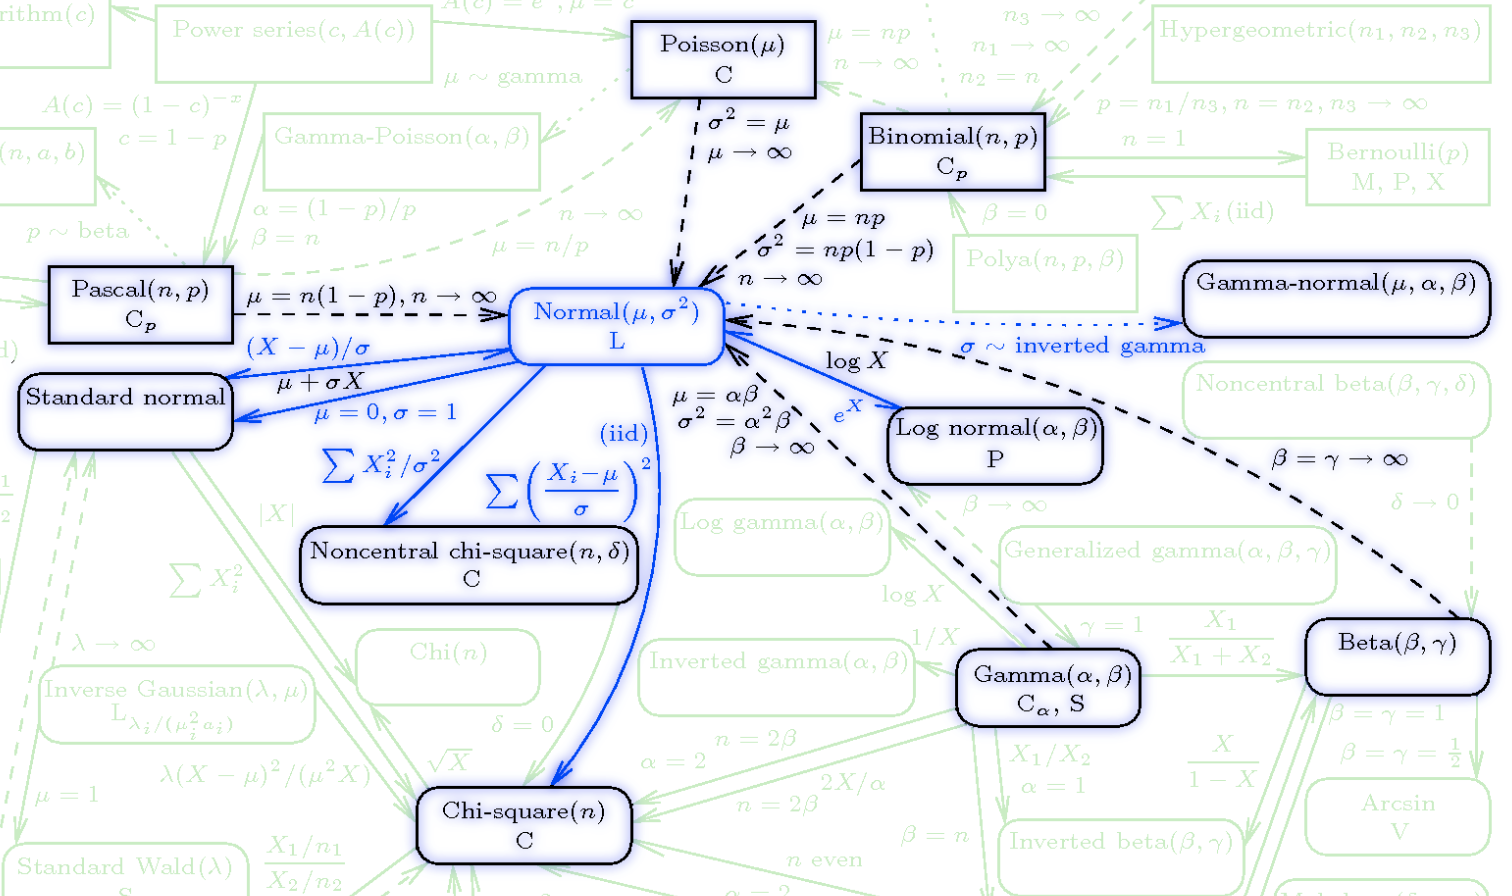
\includegraphics[height=10cm]{UDR.png}
\caption{\tiny{A snapshot of the UDR shows how the normal distribution can be transformed into a multitude of other distributions.}}
\end{figure}

\tiny{Hakaru functions representing probabilistic models (i.e. functions with a {\tt \tiny{measure(<type>)}} return type) cannot be used as operands in normal mathematical operations. This is to say we cannot transform models directly (i.e. we can’t do algebraic transformation on the PDF). The only operator we can use on a model is bind ({\tt \tiny{<$\sim$}}), to pull a sample from it. However, we are able to transform samples however we like. Therefore, we are interested in implementing transformations of the following form.}

\begin{equation*}
\begin{aligned}
& \tcboxmath[boxrule=2pt,colframe=MacMaroon]{R(p, q) \Rightarrow \textit{X} \sim A(p) \Rightarrow \textit{f(X)} \sim B(q)}
\end{aligned}
\end{equation*}

\bigskip

\tiny{In the equation above, \textit{p} is a set of values parameterizing the distribution \textit{A}}, \textit{q} is a set of values parameterizing the distribution \textit{B}, \textit{R(p, q)} is a set of relationships between \textit{p} and \textit{q} that must be satisfied, and \textit{f} is a function that applies a transformation to a sample. We can expand this definition to include transformations defined in terms of an aggregation of multiple independent samples. For example, the standard chi-square distribution is defined as the sum of the squares of \textit{n} standard normal random variables. 

\bigskip

\tiny{Hakaru also lends itself very well to Bayesian transformations where we want to pull a sample from a distribution which is parameterized with a value sampled from another distribution. These transformations take the following form. Here, we are saying that if \textit{X} is parameterized by \textit{p}, then the distribution \textit{C}, which is parameterized by \textit{p} and \textit{q}, is equal to another distribution, \textit{Y}, which is parameterized by \textit{q} and \textit{X}.}

\begin{equation*}
\begin{aligned}
& \tcboxmath[boxrule=2pt,colframe=MacMaroon]{X \sim A(p) \Rightarrow C(p, q) = Y \sim B(q, X)}
\end{aligned}
\end{equation*}

\bigskip

Some distributions on the UDR are unreachable from Hakaru's primitive distributions using transformations like the 2 described above. In these cases, we have to implement the model in terms of the PMF for a discrete distribution or in terms of the PDF for a continuous distributions. We now discuss this process in the following examples. 

\end{block}

\end{textblock}

\end{textblock}


\begin{textblock}{5}(10.75,4)

%%%%%%%%%%%%%%%%%%%%%%%%%%%%%%%%%%%%%%%%%%%%%%%%%%%%%%%%%%%%%%%%%%%%%%
% Testing Relationships Between Distributions
%%%%%%%%%%%%%%%%%%%%%%%%%%%%%%%%%%%%%%%%%%%%%%%%%%%%%%%%%%%%%%%%%%%%%%

\begin{variableblock}{}{}{}
\justifying

\small{\textbf{Discrete Distributions from PMF}}

\bigskip

\tiny{When the PMF implies a finite number of categories, the use of the primitive {\tt \tiny{categorical}} distribution combined with the array constructor language feature lends itself very well to an implementation of the distribution. However, discrete distributions have PMFs implying an infinite number of categories. This can’t be implemented using {\tt \tiny{categorical}}, which requires a finite size array. In this case, we use the {\tt \tiny{weight}} function primitive to Hakaru. The {\tt \tiny{weight}} function assigns a weight to each sample. Shown below is an example using the {\tt \tiny{weight}} function.
}

\begin{center}
\justifying
~~~~~~~~~~~~~~~~~~~~~~~~~~\tt{ \small{burglary {\color{green}<$\sim$} {\color{blue}categorical}([{\color{purple}0.0001}, {\color{purple}0.9999}])}}

~~~~~~~~~\tt{\small{{\color{blue}weight}([{\color{purple}0.95}, {\color{purple}0.01}][burglary],}}

~~~~~~~~~\tt{\small{{\color{red}return} [{\color{red}true},{\color{red}false}][burglary])}}
\end{center}

\bigskip

\tiny{In this example, the value {\tt \tiny{burglary}} is sampled from a {\tt \tiny{categorical}} distribution. Then, the samples are reweighted so that {\tt \tiny{true}} has a weight of $0.95$ and {\tt \tiny{false}} has a weight of 0.01. For the distribution samplings that are implemented in the standard library, the first argument is the PMF or PDF of the distribution and the second argument is the random variable. For example the following is the code that implements a model of the discrete Weibull distribution}

\begin{center}
\justifying
~~~~~~~~~~~~~~~~~\tt{\small{{\color{red}def} {\color{blue}discreteWeibull}(p {\color{green}prob}, beta {\color{green}prob}):}}

~~~~~~~~\tt{\small {x {\color{green} <$\sim$} {\color{blue} counting}()}}

~~~~~~~~\tt{\small{{\color{blue}weight}({\color{red}if} (x {\color{green}<} {\color{purple}0}):~{\color{purple}0} {\color{red}else}:~({\color{purple}1}~{\color{green}-}~p)~{\color{green}**}~(x~{\color{green}**}~beta) }}

~~~~~~~~~~~~~~~\tt{\small{{\color{green}-} ({\color{purple}1~}{\color{green}-}~p){\color{green}~**~}((x{\color{green}~+}{\color{purple}~1}){\color{green}~**~}beta), {\color{red}return} x)}}
\end{center}

\bigskip

\tiny{The first line of code in the function definition, {\tt \tiny{x <$\sim$ counting()}}, assigns an integer to \textit{x} according to a uniform distribution across all integers.
The first argument of {\tt \tiny{weight}} is the PMF of the distribution and the second argument is the random variable. In this way, each instance of the random variable is given a weight equal to that instance's probability.
}

\small{\textbf{Continuous Distributions from PMF}}

\bigskip

\tiny{This is accomplished similar to how discrete distributions with infinite categories implied by their PMF are implemented. The main difference is that the {\tt \tiny{lebesgue}} function is used instead of {\tt \tiny{counting}} to sample values from the real number line.}


\end{variableblock}

%%%%%%%%%%%%%%%%%%%%%%%%%%%%%%%%%%%%%%%%%%%%%%%%%%%%%%%%%%%%%%%%%%%%%%
% Testing Relationships Between Distributions
%%%%%%%%%%%%%%%%%%%%%%%%%%%%%%%%%%%%%%%%%%%%%%%%%%%%%%%%%%%%%%%%%%%%%%

\begin{block}{Testing Relationships Between Distributions}
\justifying

\tiny{Recall that when developing the standard library, the UDR chart often implied multiple possible implementations for a given distribution. Naturally, we would expect alternative implementations for the same distribution to result in equivalent probabilistic models. This line of thought is the basis for the kinds of test cases we have implemented. More generally, we have the following hypothesis.}

\bigskip

\tiny{Assume we know a proven relationship between 2 statistical distributions, A and B, which allows us to transform A and B into distributions that are equivalent to each other. Further assume this transformation takes on one of the forms discussed in the Standard Library Development section. We hypothesize that by applying the appropriate transformations to implementations of A and B, we can create two Hakaru programs whose `hk-maple' outputs will be equivalent to each other. Test cases that prove our hypothesis true indicate the validity of the Hakaru language implementation. Test cases that prove our hypothesis false indicate an underlying bug in the language definition which is to be passed back to the language developers.
}

\end{block}

%%%%%%%%%%%%%%%%%%%%%%%%%%%%%%%%%%%%%%%%%%%%%%%%%%%%%%%%%%%%%%%%%%%%%%
% Conclusions & Future Work
%%%%%%%%%%%%%%%%%%%%%%%%%%%%%%%%%%%%%%%%%%%%%%%%%%%%%%%%%%%%%%%%%%%%%%

\begin{block}{Conclusions \& Future Work}

Conclusions \& Future Work

\end{block}

%%%%%%%%%%%%%%%%%%%%%%%%%%%%%%%%%%%%%%%%%%%%%%%%%%%%%%%%%%%%%%%%%%%%%%
% References
%%%%%%%%%%%%%%%%%%%%%%%%%%%%%%%%%%%%%%%%%%%%%%%%%%%%%%%%%%%%%%%%%%%%%%

\begin{block}{References}

References

\end{block}


% \begin{block}{References}
% \setbeamertemplate{bibliography item}{\insertbiblabel}
% \bibliographystyle{ieeetr}
% {\scriptsize
% \bibliography{../bib}}
% \end{block}

\end{textblock}
\end{frame}
\end{document}
